\pagebreak
\section{Friction test} %\label{put a label here and uncomment}
\textbf{Name: Group 510}\\
\textbf{Date: 28/10 - 2015}

\subsection{Purpose}
The purpose of the test is to find the total friction, $B$, of the vehicle.

\subsection{Setup}
\begin{figure}[H]
  \centering
	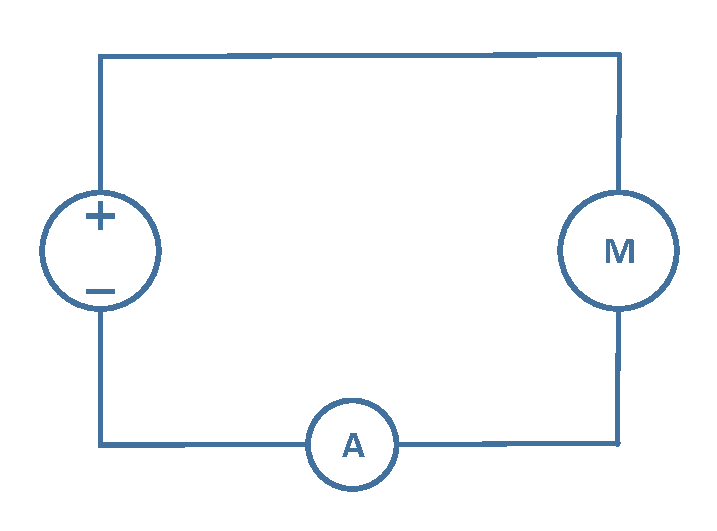
\includegraphics[scale=0.5]{figures/FrictionTest.pdf}
	\caption{A diagram of the test setup}
\end{figure}

\subsection{List of Equipment}

\begin{table}[H]
\begin{tabular}{|l|l|p{4cm}|}
\hline%------------------------------------------------------------------------------------
  \textbf{Instrument}                       &  \textbf{AAU-no.}  &  \textbf{Type}         \\
\hline%------------------------------------------------------------------------------------
  Multimeter                                &  60764             &  Fluke 189 true RMS    \\
\hline%------------------------------------------------------------------------------------
  Power Supply ($0 - 32$ V) ($0 - 10$ A)    &  77075             &  Ea - ps 7032 - 100    \\
\hline%------------------------------------------------------------------------------------
  Treadmill                                 &  75483             &  Rodby                 \\
\hline%------------------------------------------------------------------------------------
\end{tabular}
\end{table}

\subsection{Procedure}

\begin{enumerate}
  \item Connect the power supply's power channel to the motor and the ground channel to the multimeter.
  \item Place the vehicle in the middle of the treadmill.
  \item Set the power supply to current limiting at a maximum of $4$ amperes, the vehicle is not running, but ready to run when the power supply is set above $4$ amperes later. 
  \item Activate the treadmill to run at the required speed, and at the same time correct the power supply so the vehicle receives more than $4$ amperes and thereby making it move.
  \item Correct the speed of the vehicle with the power supply until the vehicle has the same velocity as the treadmill.
  \item Read the current on the multimeter.
  \item Repeat the process with different velocities.
\end{enumerate}

\subsection{Results}
The raw data extracted from the measurements is the vehicle's velocity in $[km \cdot h^{-1}]$ and the current needed for achieving the specific velocity. The velocity is calculated from $[km \cdot h^{-1}]$ to a linear velocity $[m \cdot s^{-1}]$:

\begin{flalign}
\eq{V}{\frac{V_m \cdot 10^{3}}{3600}} \unit{m \cdot s^{-1}}
\end{flalign}
\hspace{6mm} Where:\\
\begin{tabular}{p{1cm}lll}
& $V_m$ & is measured velocity of the vehicle &\unitWh{km \cdot h^{-1}}\\
& $V$   & is the vehicle's linear velocity    &\unitWh{m \cdot s^{-1}}\\
\end{tabular}

By using linear velocity $[m \cdot s^{-1}]$, the motor's angular velocity $[rad \cdot s^{-1}]$ can be calculated:

\begin{flalign}
\eq{\omega_m}{\frac{V \cdot N}{r_t}} \unit{rad \cdot s^{-1}}
\end{flalign}
\hspace{6mm} Where:\\
\begin{tabular}{p{1cm}lll}
& \si{\omega_m} & is the motor's angular velocity                   &\unitWh{\frac{rad}{s}}\\
& $N$           & is the gear ratio of the vehicle                  &\unitWh{\cdot}\\
& $r_t$         & is the radius of the two wheels driving the belts &\unitWh{m}\\
\end{tabular}

The motor's torque and angular velocity is plotted: 

\begin{figure}[H]
  \centering
	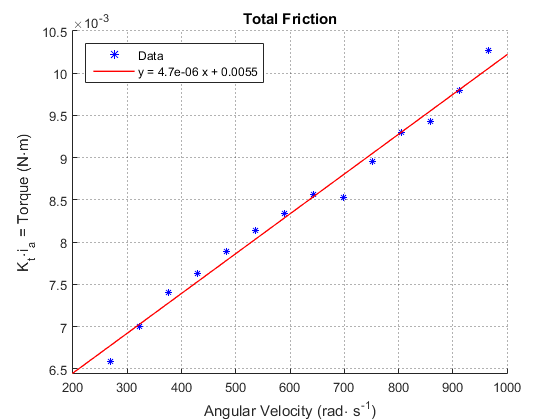
\includegraphics[scale=1]{figures/FrictionTestPlot.png}
	\caption{A plot of the motor's torque over the motor's angular velocity. The blue dots indicates the measurements and the red line is the tendency line.}
	\label{TotalFriction}
\end{figure}

The red line in \figref{TotalFriction} is the tendency line, the slope indicates the friction and the offset is the stiction of the system. The total friction of the system is therefore:

\begin{flalign}
\eq{B_{tot}}{4.7 \cdot 10^{-6}} \ \si{N \cdot m \cdot rad^{-1} \cdot s}&
\end{flalign}